% This is the Reed College LaTeX thesis template. Most of the work 
% for the document class was done by Sam Noble (SN), as well as this
% template. Later comments etc. by Ben Salzberg (BTS). Additional
% restructuring and APA support by Jess Youngberg (JY).
% Your comments and suggestions are more than welcome; please email
% them to cus@reed.edu
%
% See http://web.reed.edu/cis/help/latex.html for help. There are a 
% great bunch of help pages there, with notes on
% getting started, bibtex, etc. Go there and read it if you're not
% already familiar with LaTeX.
%
% Any line that starts with a percent symbol is a comment. 
% They won't show up in the document, and are useful for notes 
% to yourself and explaining commands. 
% Commenting also removes a line from the document; 
% very handy for troubleshooting problems. -BTS

% As far as I know, this follows the requirements laid out in 
% the 2002-2003 Senior Handbook. Ask a librarian to check the 
% document before binding. -SN

%%
%% Preamble
%%
% \documentclass{<something>} must begin each LaTeX document
\documentclass[12pt,twoside]{reedthesis}
% Packages are extensions to the basic LaTeX functions. Whatever you
% want to typeset, there is probably a package out there for it.
% Chemistry (chemtex), screenplays, you name it.
% Check out CTAN to see: http://www.ctan.org/
%%
\usepackage{graphicx,latexsym} 
\usepackage{amssymb,amsthm,amsmath}
\usepackage{longtable,booktabs,setspace} 
%\usepackage{chemarr} %% Useful for one reaction arrow, useless if you're not a chem major
\usepackage{url}
\usepackage{natbib}
% \usepackage{times} % other fonts are available like times, bookman, charter, palatino

\newcommand{\eqn}[1]{\begin{equation}#1\end{equation}}
\newcommand{\eq}[1]{\begin{align}#1\end{align}}


\title{Quantum Mechanical Bound States of the Yukawa Potential (or some better title)}
\author{Ellen M. McManis}
% The month and year that you submit your FINAL draft TO THE LIBRARY (May or December)
\date{May 2012}
\division{Mathematics and Natural Sciences}
\advisor{Nelia Mann}
%If you have two advisors for some reason, you can use the following
%\altadvisor{Your Other Advisor}
%%% Remember to use the correct department!
\department{Physics}
% if you're writing a thesis in an interdisciplinary major,
% uncomment the line below and change the text as appropriate.
% check the Senior Handbook if unsure.
%\thedivisionof{The Established Interdisciplinary Committee for}
% if you want the approval page to say "Approved for the Committee",
% uncomment the next line
%\approvedforthe{Committee}

\setlength{\parskip}{0pt}
%%
%% End Preamble
%%
%% The fun begins:
\begin{document}

  \maketitle
  \frontmatter % this stuff will be roman-numbered
  \pagestyle{empty} % this removes page numbers from the frontmatter

% Acknowledgements (Acceptable American spelling) are optional
% So are Acknowledgments (proper English spelling)
    \chapter*{Acknowledgements}
	People. Things. Shep, the dog who is currently keeping me company.

% The preface is optional
% To remove it, comment it out or delete it.
%    \chapter*{Preface}
%	This is an example of a thesis setup to use the reed thesis document class.

    \tableofcontents
% if you want a list of tables, optional
    \listoftables
% if you want a list of figures, also optional
    \listoffigures

% The abstract is not required if you're writing a creative thesis (but aren't they all?)
% If your abstract is longer than a page, there may be a formatting issue.
    \chapter*{Abstract}
	Math and computers and stuff gave me results!
		
%	\chapter*{Dedication}
%	You can have a dedication here if you wish.

  \mainmatter % here the regular arabic numbering starts
  \pagestyle{fancyplain} % turns page numbering back on

%The \introduction command is provided as a convenience.
%if you want special chapter formatting, you'll probably want to avoid using it altogether

    \chapter*{Introduction}
         \addcontentsline{toc}{chapter}{Introduction}
	\chaptermark{Introduction}
	\markboth{Introduction}{Introduction}
	% The three lines above are to make sure that the headers are right, that the intro gets included in the table of contents, and that it doesn't get numbered 1 so that chapter one is 1.

% Double spacing: if you want to double space, or one and a half 
% space, uncomment one of the following lines. You can go back to 
% single spacing with the \singlespacing command.
% \onehalfspacing
% \doublespacing
The Yukawa potential describes a force mediated by a massive particle. It is %argh fuck this part
\eqn{
V(r) = -\frac{C}{r}e^{-r/l}\mbox{,}
}
where $C$ and $l$ are constants. $C$ sets the strength of the force; $l$ acts as a length scale. The exponential term provides an effective cutoff once $r$ gets much larger than $l$, as the exponential term drops off quite rapidly. We are interested in how the bound states change with these constants. 

The force described by the potential comes from the exchange of virtual particles. The lenth scale, which limits the range at which the force acts, comes about because the virtual particles exchanged have mass. The mass of these particles then generates the length scale:
\eqn{
l = \frac{\hbar}{m_{\pi}c}\mbox{.}
}
The strength of the force $C$ is only known experimentally and depends on the application of the potential. Most commonly, this is the forces between protons and neutrons in an atomic nucleus.

In general, the time-independent Schr\"odinger wave equation for some $V(r)$ is
\eqn{
-\frac{\hbar^2}{2\mu}\nabla^2\psi(r,\phi,\theta) + V(r)\psi (r,\phi,\theta) = E \psi(r,\phi,\theta)\mbox{.}
\label{eq:TIDSWE-general}
}
In this thesis, we work with a system of two particles moving under the influence of the Yukawa potential (in the atomic case, this would be a deuterium nucleus). To simplify the system, it makes the most sense to express this in spherical coordinates as a reduced mass orbiting a center of mass. This is the form used for the wave equation above. With the Yukawa potential, this equation cannot be solved analytically. However, we can solve the more simple system described by the potential without the exponential term, that is,
\eqn{
 V(r) = -\frac{C}{r}\mbox{.}
 }
This potential is the same form as the Coulomb potential in the hydrogen atom. While $r << l$, the Yukawa potential should behave similarly to this, because the $-C/r$ term will dominate. Therefore, we will gain some insight on the Yukawa potential by solving the wave equation for this one.
The Schr\"odinger wave equation with this simpler potential can be solved analytically by separation of variables. While the final wave function will be dependent on all three variables, the energy is just a function of $n$ (the radial quantum number), and is equal to
\eqn{
E_n = -\frac{\mu e^4}{(4 \pi \epsilon_0)^2 2 \hbar ^2 n^2}\mbox{.}
\label{eq:hydrogen-E}
}
This can be rewritten in terms of 
\eqn{
a_0 \equiv \frac{4 \pi \epsilon_0 \hbar ^2}{\mu e^2}\mbox{,}
}
the ``Bohr radius". A constant with units of length, $a_0$ is defined in terms of the other constants in the problem. It is also equal to the radius of the smallest orbit in a Bohr hydrogen atom (the ground state). As such, it sets a natural length scale. Substituting $a_0$ in, the expression for $E_n$ becomes much simpler:
\eqn{
E_n = -\frac{\hbar^2}{a_0^2 \mu n^2}\mbox{.}
\label{eq:hydrogen-Ebohr}
}
These energies are the energies of the bound states of the electron in the hydrogen atom. As $n$ increases, $E_n$ gets closer and closer to zero, but never quite reaches it -- there are an infinite number of bound states possible.
\begin{figure}
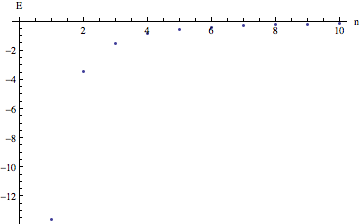
\includegraphics[scale=0.75]{hydrogenspectrum.png}
\caption{The energies of the first 10 bound states of the electron in the hydrogen atom}
\label{fig:hspec}
\end{figure}

The ground state wave function is spherically symmetric, meaning that $\psi$ there is only a function of $r$. This function is plotted in Figure \ref{fig:hground}.

\begin{figure}
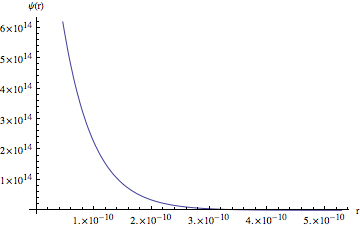
\includegraphics[scale=0.75]{hydground.png}
\caption{The ground state ($n=1$, $l =0$, $m= 0$) wave function for hydrogen}
\label{fig:hground}
\end{figure}

This means the Yukawa potential's range is limited in a way the Coulomb potential's isn't. We expect that this will limit the number of bound states as well, to some number whose $r$s are less than $l$.
%\clearpage %% starts a new page and stops trying to place floats such as tables and figures
%
%
%\chapter*{Conclusion}
%         \addcontentsline{toc}{chapter}{Conclusion}
%	\chaptermark{Conclusion}
%	\markboth{Conclusion}{Conclusion}
%	\setcounter{chapter}{4}
%	\setcounter{section}{0}
%	
%
%%If you feel it necessary to include an appendix, it goes here.
%    \appendix
%      \chapter{The First Appendix}
%      \chapter{The Second Appendix, for Fun}
%
%
%%This is where endnotes are supposed to go, if you have them.
%%I have no idea how endnotes work with LaTeX.
%
\backmatter % backmatter makes the index and bibliography appear properly in the t.o.c...
%
% Make my bibliography be called "Bibliography" and not "References" (or "Works Cited" or...):
%% \renewcommand{\bibname}{Works Cited}

 \bibliographystyle{plain}
%FIXME: should be apsrev.
  
% there are a variety of styles available; 
%% replace ``plainnat'' with the style of choice. You can refer to files in the bsts or APA 
%% subfolder, e.g. 
%% \bibliographystyle{APA/apa-good}  % or
%% \bibliographystyle{bsts/mla-good} 
%
%% if you're using bibtex, the next line forces every entry in the bibtex file to be included
%% in your bibliography, regardless of whether or not you've cited it in the thesis.
   \nocite{*}
   \bibliography{em_thesis}

% Finally, an index would go here... but it is also optional.
\end{document}
